% !TEX root = ../thesis.tex

\chapter{Celkové vyhodnotenie}

V tejto práci sme uviedli spôsob vykonávania a merania kvantových obvodov.
Využitím vedomostí z matematiky a funkcionálneho programovania sme úspešne 
navrhli a implementovali model pre počítanie fiktívnych meraní kvantových
bitov v kvantových obvodoch.

I keď nie je možné porovnávať simulátor kvantového stroje IBM Quantum
Experience s pravdepodobnostným modelom je nutné vyzdvihnúť fakt, že k
výsledkom a teda k predstave ako prebieha kvantový program sa dostaneme 
oveľa rýchlejšie. Na obrázku \ref{expr_time} sú zobrazené výpisy o dokončení
meraní experimentu v IBM QX. Pri experimentoch, ktoré sme vykonávali sme 
robili štyri fiktívne merania. Pre zistenie výsledkov zo simulátora kvantového
stroja, bolo nutné vykonať jednotlivé merania osobitne a to zabralo relatívne
veľa času. Ako je vidno na obrázku (\ref{expr_time}), vykonanie štyroch 
takýchto meraní trvalo viac ako dve minúty. Kde náš pravdepodobnostný model
vďaka tomu, že nemusí robiť reálne meranie ale len to fiktívne, vracia 
výsledky okamžite. 

\begin{figure}
	\centering 
	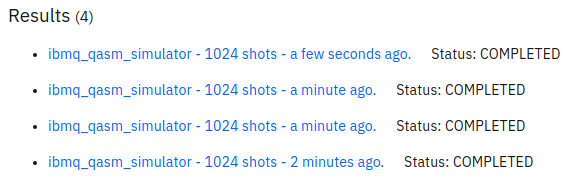
\includegraphics[width=.8\textwidth]{figures/time_expr.png} 
	\caption{Časy dokončení meraní experimetov.}
    \label{expr_time}
\end{figure}


Samozrejme, že ak potrebujeme presné merania, je lepšie použiť kompletný
simulátor. No výhodou nášho riešenia je zobrazenie zmien stavov kvantových
bitov. IBM QX dokáže zobraziť len skolabované výsledky meraní, i keď veľmi
presne, no niekedy je vhodnejšie vedieť stav ešte pred kolabovaním. Náš 
pravdepodobnosný model generuje stromovú štruktúru, v ktorej si zaznamenáva
priebežné stavy kvantových bitov. Získané stromy z našich experimentov sme 
pridali do príloh tejto práce.

Funkčnosť modelu sme otestovali na troch experimetoch. V každom experimente 
sme odvodili vzorce pre výpočet pravdepodobností kolabovania do jednotlivých
stavov pre všetky definované časové okamihy. Uviedli sme výsledky, ktoré 
sú dosiahnuteľné pomocou kvantového stroja IBM Quantum Experience. Nakoniec 
sme pre každý experiment uskutočnili meranie pomocou nášho pravdepodobnostného
modelu.

V neposlednej rade sme preskúmali aj možnosť využitia tohto pravdepodobnostného
modelu aj pri zložitejšom príklade, v ktorom prebiehal kvantový jaz zvaný
kvantová teleportácia.
